\chapter{Short Read Structural Variation Detection and Characterization Using Convolutional Neural Networks}

\section{Introduction}

Genomic structural variation, broadly defined as genetic polymorphisms larger than 50bp, are an increasingly prevalent area of study in medical, agricultural, and ecological contexts \cite{sudmantIntegratedMapStructural2015,duAnalysisStructuralVariants2021,weissensteinerDiscoveryPopulationGenomics2020,chakrabortyEvolutionGenomeStructure2021,chakrabortyHiddenGeneticVariation2018,merkerLongreadGenomeSequencing2018,bickhartChallengesImportanceStructural2014}. Structural variation has traditionally been a difficult aspect of the genome to detect and characterize with commonly used short-read sequencing approaches, though a variety of methods have been developed in attempt to increase detection power \cite{clealDysguEfficientStructural2022,rauschDELLYStructuralVariant2012,chenMantaRapidDetection2016,belyeuSamplotPlatformStructural2021,popicCueDeeplearningFramework2023}(reviewed in \cite{cameronComprehensiveEvaluationCharacterisation2019}, \cite{mahmoudStructuralVariantCalling2019} and \cite{alkanGenomeStructuralVariation2011}). Long-read genome sequencing methods have become the \textit{de facto} approach for highly accurate structural variant calling but remain a relatively expensive and low-throughput method compared to short-read sequencing \cite{merkerLongreadGenomeSequencing2018,dierckxsensBenchmarkStructuralVariation2021,chenDecipheringExactBreakpoints2023,ahsanSurveyAlgorithmsDetection2023,decosterPopulationscaleLongreadSequencing2021}, especially in the context of population genetics where larger sample sizes are necessary to facilitate more accurate approximations of a variant's frequency within a population. It is therefore advantageous to create methods that can accurately detect and characterize structural variation from short-read sequencing data that can be applied to readily available short-read sequencing data for population genetics-scale analysis of structural variation.

Deep learning has been shown to successfully detect single nucleotide polymorphisms (SNPs) \cite{poplinUniversalSNPSmallindel2018}, and there has even been success in structural variation detection \cite{popicCueDeeplearningFramework2023,hillDeepLearningApproach2019}, but current attempts continue to fail to meet the benchmarks set by long-read approaches. Convolutional neural networks (CNNs) extract features that they “learn” to be important for various classifications and make decisions based on said features \cite{liSurveyConvolutionalNeural2022,lecunBackpropagationAppliedHandwritten1989,lecunGradientbasedLearningApplied1998}. They can classify an image based on patterns not readily apparent to humans or traditional methods, and therefore can draw conclusions about data that would otherwise be impossible or extremely difficult. This makes them an appealing choice for structural variation detection, provided a suitable data representation can be created to expose as much information about the underlying genetics as possible to the network.

Here we develop and report preliminary benchmarks on a novel genomic representation for structural variation detection and characterization using an ensemble approach consisting of random forests, CNNs, and object detection models. This representation proves to be highly flexible and accurate for multiple structural variant types, with the potential for improvement and adaptation to other similar areas, such as transposable elements (TEs). Our approach utilizes a core set of highly accurate long-read and short-read matched sequencing data which has had structural variants (SVs) characterized using long-read sequencing methods. This allows us to develop a model using validated locations of structural variants where short-read data is available to generate training representations. When using this model for prediction, only the short read data is then needed, allowing users of the model to accurately and quickly call SVs without needing to perform long-read sequencing, and opening up the avenue for not only population-scale analyses, but reanalysis of old data to find novel, publishable, and accurate results previously unattainable. This method aims to open up the potential for SV discovery and characterization in every genetics study that incorporates short-read sequencing.

\section{Methods}

\subsection{Data representation}

Here we expand on concepts described in \cite{hillDeepLearningApproach2019}, wherein we propose a summary vector as input features for machine learning models. This representation is composed of many features calculated on a per-base level, such that for a given base the count of reads aligned to that base that have the following qualities are enumerated in Table 3.1. For a given alignment provided as a SAM/BAM file, we first use samtools \cite{danecekTwelveYearsSAMtools2021} to extract plaintext alignment data from a query location using the target chromosome, start, and end of the queried window. For each base pair in the alignment within the query window we calculate the per-base pair sum of all features listed in Table 1 by extracting information from the CIGAR string, bitwise flag, and general alignment information reported by the SAM/BAMfile. We then calculate the mean, standard deviation, median, and interquartile range (IQR) for each statistic across the region, resulting in a concise vector representation of relevant features for a given region of the genome. This process of feature vector conversion is parallelized at the thread level, allowing for fast computation of population-scale feature vectors given a read alignment file. We find different feature distributions for different SV types, exemplified in Figure \ref{fig:read-dists}.

\begin{figure}
    \centering
    \makebox[\textwidth][c]{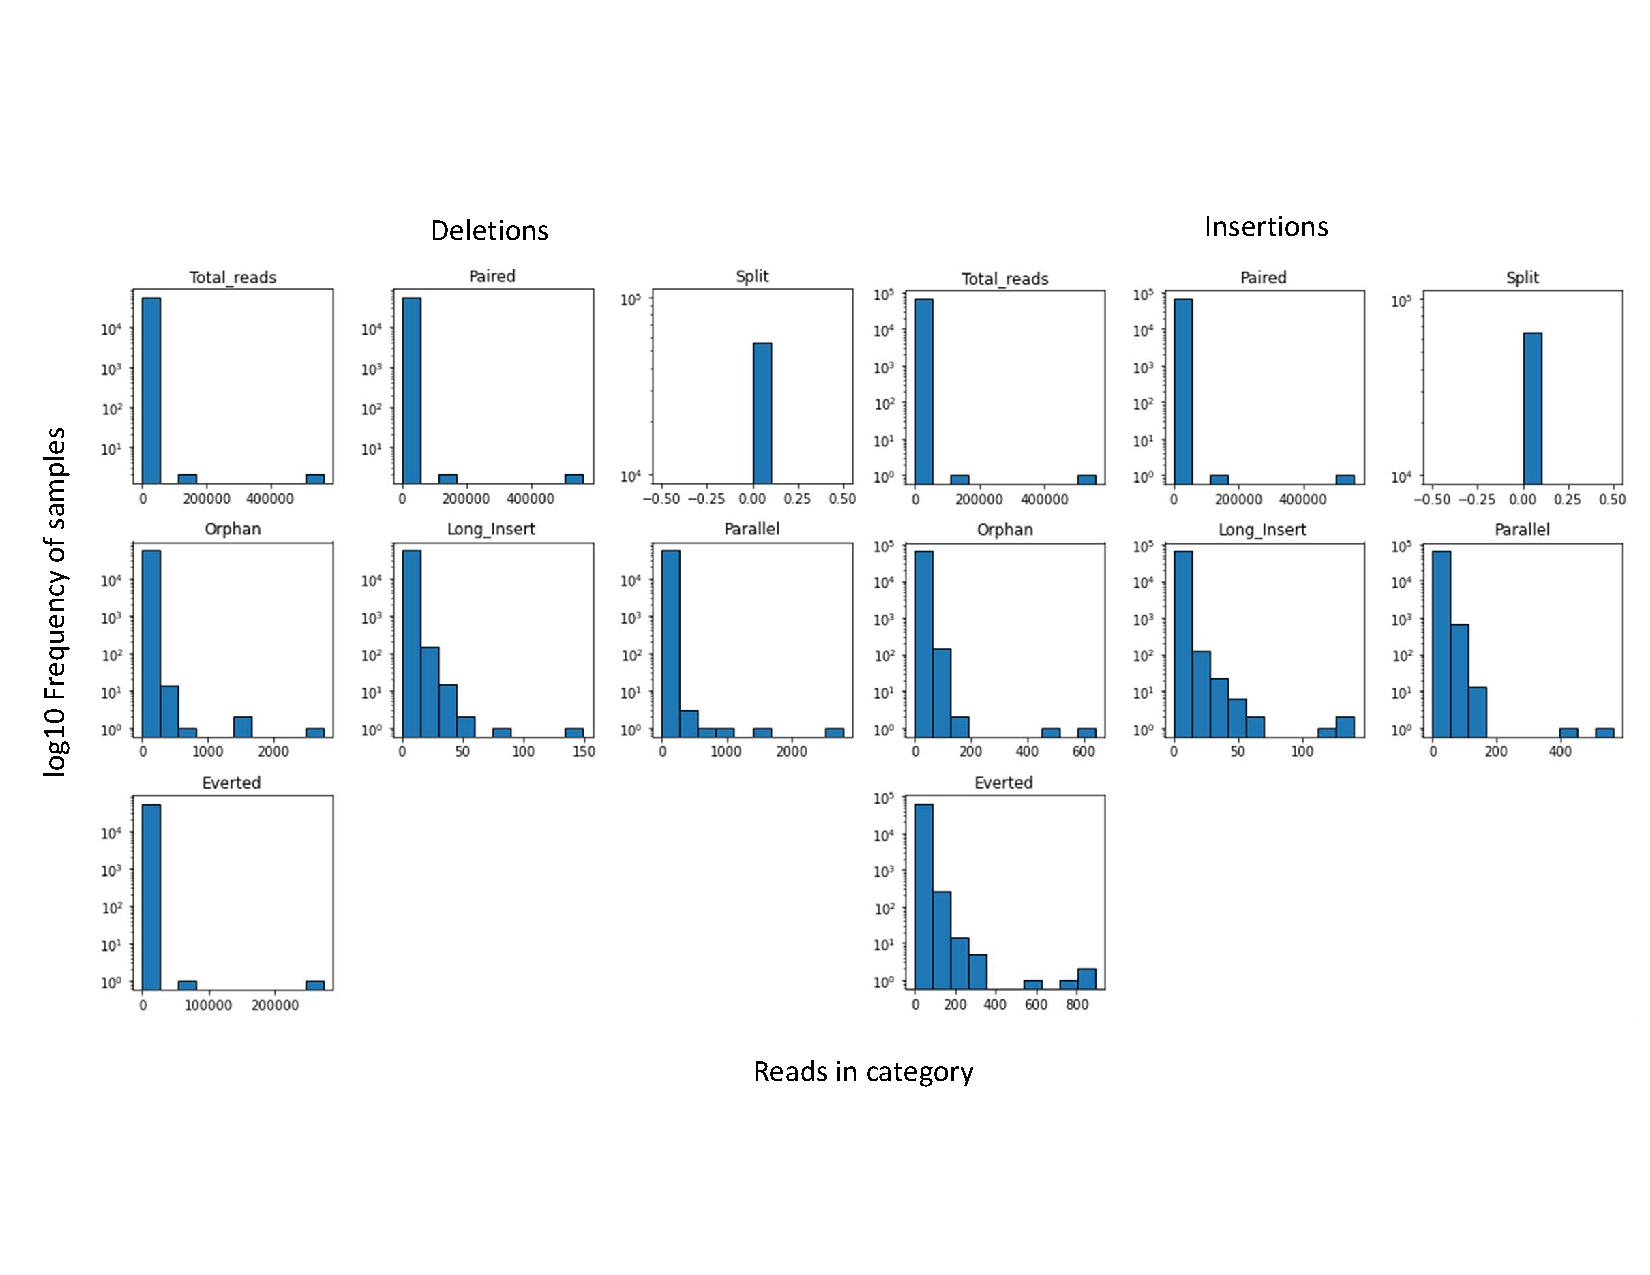
\includegraphics[width=\textwidth]{figures/ch3/read_type_distribution.pdf}}
    \caption[Distribution of read flags per structural variant type.]{Distribution of read flags per structural variant type.}
    \label{fig:read-dists}
\end{figure}

\begin{table}[htb]
\resizebox{\textwidth}{!}{%
\begin{tabular}{|l|l|}
\hline
Feature              & Description                                                                                                              \\ \hline
Paired               & Whether the read is single or paired                                                                                     \\ \hline
Proper\_Pair         & Whether the read pair is mapped in the correct order (first read comes before the second in terms of genome coordinates) \\ \hline
Is\_Read1\_Unmapped  & Is the first read unmapped                                                                                               \\ \hline
Is\_Read2\_Unmapped  & Is the second read unmapped                                                                                              \\ \hline
Is\_Read1\_Rev\_Comp & Is the first read reverse complement of the reference                                                                    \\ \hline
Is\_Read2\_Rev\_Comp & Is the second read reverse complement of the reference                                                                   \\ \hline
Is\_First\_Read      & Binary flag for first read                                                                                               \\ \hline
Is\_Second\_Read     & Binary flag for second read                                                                                              \\ \hline
Split                & Is the read non-contiguous (suggesting an insertion within the read itself)                                              \\ \hline
Long\_Insert         & Is the gap between the read pair larger than the 99th percentile of insert lengths across the alignment                  \\ \hline
Short\_Insert        & Is the gap between the read pair smaller than the 2nd percentile of insert lengths across the alignment                  \\ \hline
Parallel\_Read       & Do both reads of the read pair align to the same orientation of the genome                                               \\ \hline
Everted\_Read        & Are the reads in the pair facing away from each other as opposed to towards each other                                   \\ \hline
Orphan\_Read         & Is this read flagged as paired end but the pair does not align to the reference                                          \\ \hline
\end{tabular}%
}

\caption{List of features included in short-read alignment feature respresentation and their description.}

\end{table}

\subsection{Data retrieval and preprocessing}
Data for this study was collected from \textit{Drosophila melanogaster} assemblies and sequencing runs as reported in \cite{chakrabortyEvolutionGenomeStructure2021,chakrabortyHiddenGeneticVariation2018,chakrabortyStructuralVariantsExhibit2019}. In total fourteen \textit{de novo} genome assemblies and associated structural variation callsets (detected using SVMU as described in \cite{chakrabortyStructuralVariantsExhibit2019}) were downloaded. Using the genomic coordinates obtained from the SVMU calls we prepared feature vector representations for all deletions, insertions, copy number variants, and inversions as well as control regions using the representation as described above. We then separated out one of the assemblies and callsets to serve as a hold-out test set for all analyses, hereby named the "true test set".

\subsection{Random forest classifier training}

We implemented a random forest classifier \cite{ho1995random} implemented in scikit-learn \cite{scikit-learn} with 500 estimators as a 5-class classifier, the output classes being control (no SV present), deletion, insertion, copy number variant (CNV), and inversion. Training data was split into a 77\%/33\% train/test split stratified by class labels for equal distribution between the sets. The random forest was fit to the resulting training data and validated on the test data before being applied to hold-out true test set.

\subsection{Object detection model and breakpoint identification}

To detect where SVs and their breakpoints occur in a callset we attempted to use an object detection model (https://github.com/ultralytics/yolov5). This is a form of convolutional neural network that draws boundary boxes and classifies each candidate box, allowing for precise identification of an object and its location within an image. The data representation for object detection is similar to that described in Data retrieval and preprocessing, however instead of summing features as summaries we instead represented each feature as a histogram count of the feature, with the minimum and maximum values of each being standardized across the target region. An example feature map for this data type can be seen in Figure \ref{fig:example_pileup}. 

We attempted two variants of object detection: detecting the entire SV (or in the case of an image not capturing the entire SV, what is present), and identifying breakpoints. In the case of whole-SV detection breakpoints were treated as the left and right bounds for the bounding box values and the entire y-axis was used as the vertical bounds. Bounding box values were scaled relative to 0-1 as described in the YOLOv5 tutorial based on the length of the genomic region represented scaled to a consistent image size of 640 $\times$ 640 pixels. For breakpoint detection we used a 50bp window centered on the identified breakpoint as the left and right bounds, and used the entire y-axis consistent with the entire SV approach. Both were trained under default settings for the YOLOv5s model for 3 epochs.

\begin{figure}
    \centering
    \makebox[\textwidth][c]{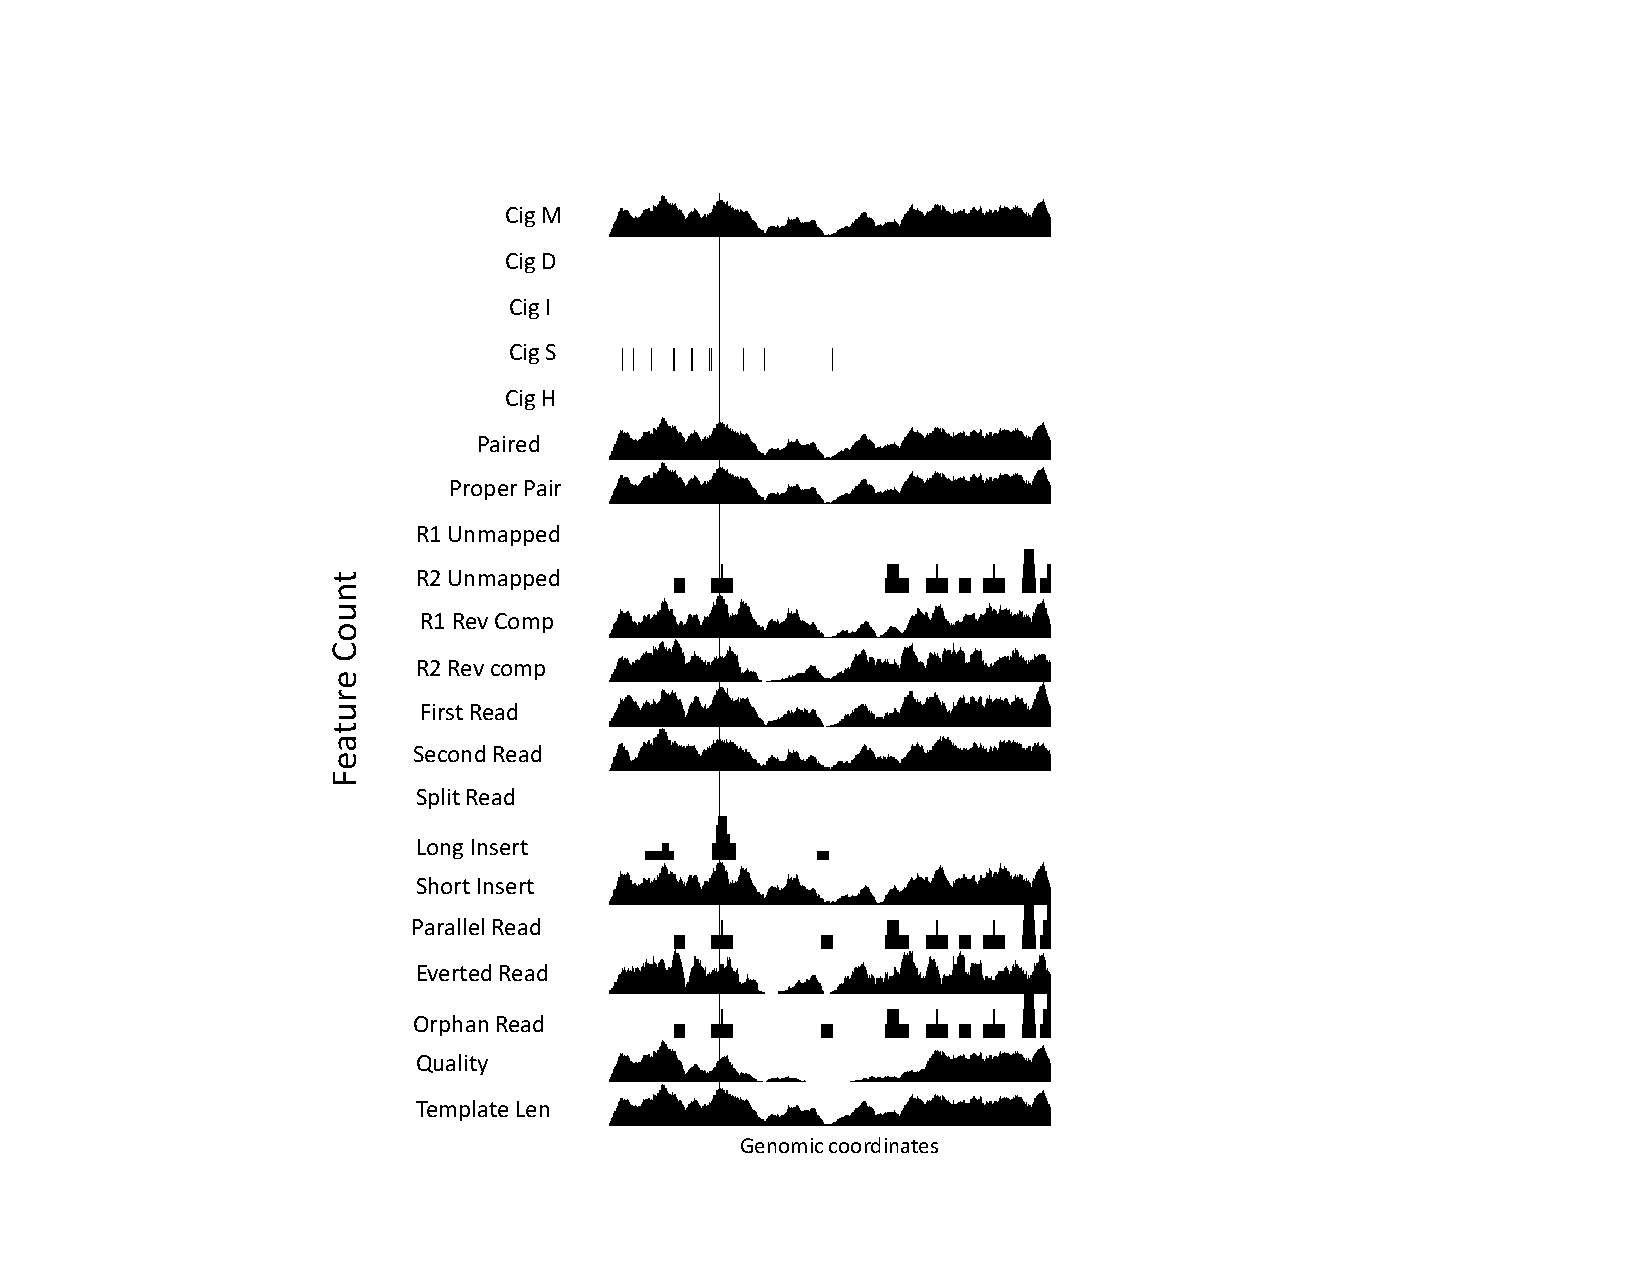
\includegraphics[width=1.5\textwidth]{figures/ch3/example_pileup.pdf}}
    \caption[Sample representations of the object detection feature matrix.]{An example of the object detection feature matrix. Grey vertical lines represent the left and right breakpoints for a candidate SV region. "Cig" is an abbreviation for CIGAR string from the SAMfile format.}
    \label{fig:example_pileup}
\end{figure}

\section{Results}

\subsection{Summarized features and random forests are a powerful method for SV classification}

To test whether our data representation of summarized features combined with random forest approaches could accurately identify and distinguish SV types we trained on a large number of long-read validated samples of structural variants in \textit{Drosophila melanogaster}. This long-read data was matched with short-read sequencing data that was used to generate feature representations from reference alignments, resulting in a training and testing set for benchmarking multiple methods on SV discovery and characterization. We find that a random forest trained on our summarized data representation achieves high levels of accuracy across multiple SV types on the true test set Figure \ref{fig:test_accuracy_forest}. One recognized caveat with this approach is the lack of substantial sample numbers for copy number variants and inversions compared to insertions and deletions, and an overall drastic imbalance of all SV types compared to control regions. This is due to three major factors; the first being that structural variants are relatively rare, and while they can span large regions of the genome, the overall composition of a given genome will largely be unaffected (control) regions. The second is that copy number variants in this instance refer to multiple duplication events, however it is possible that some CNVs are treated as insertions, this is largely a semantic difference and will change depending on how the dataset is labeled. And the final caveat is that inversions, with how drastic of an effect they have on the genome structure, are extremely rare, so they are expected to be the lowest-represented class in any given SV dataset. Multiple of these issues could be alleviated with simulated SV data, allowing for a more balanced dataset and better representation of different SV types assuming the simulated examples accurately mimic the empirical SVs.

\begin{figure}
    \centering
    \makebox[\textwidth][c]{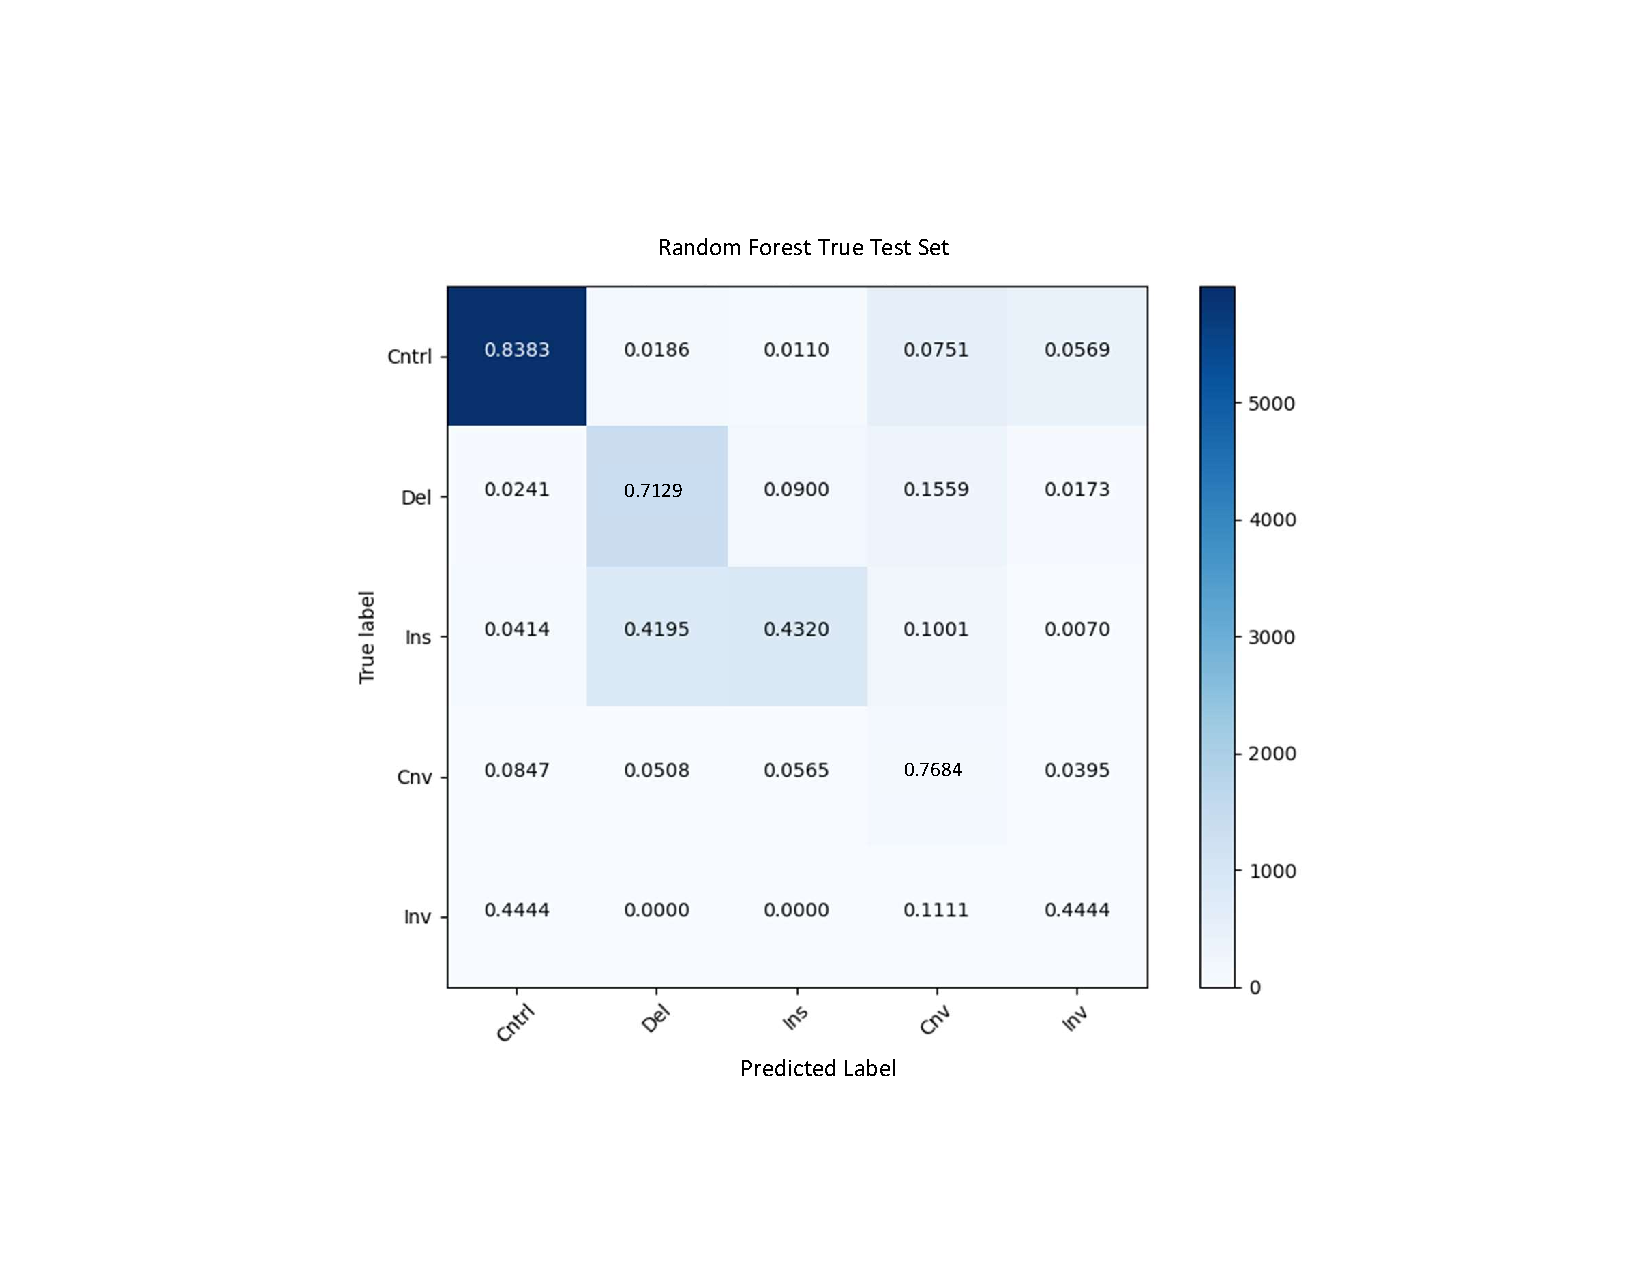
\includegraphics[width=1.5\textwidth]{figures/ch3/test_accuracy_forest.pdf}}
    \caption[Accuracy of random forest on classifying SVs on true test set.]{Accuracy of random forest on classifying SVs on true test set. Labels are controls, deletion, insertions, copy number variants, and inversions, respectively. Values are reported as proportion of true labels (along the y-axis) that are included in a given intersection. Color indicates number of samples in a given intersection scaled to the largest number of samples in a class.}
    \label{fig:test_accuracy_forest}
\end{figure}


\subsection{Random forests provide accuracy boosts when used as a filtering mechanism}

We then tested whether our random forest classifier could be used as a filtering mechanism in tandem with other short-read SV callers. We tested accuracies with and without a modified LastZ \cite{chakrabortyStructuralVariantsExhibit2019} reported candidate SVs in the true test set along with varying softmax thresholds for output probabilities counting as a positive call \ref{fig:test_accuracy_forest}. For the non-candidate examples windows of 2,500bp with 1,200bp overlap step size were extracting across the entire genome and predicted on. For LastZ candidate filtering a no-thresholding approach (any probability larger than 0.2, 1/5 classes) yields the optimal tradeoff between false positive and true negative rates. Overall performance is vastly improved by using a pre-filtering approach and treating our random forest model as a genotyper, rather than a discovery method.

\begin{figure}
    \centering
    \makebox[\textwidth][c]{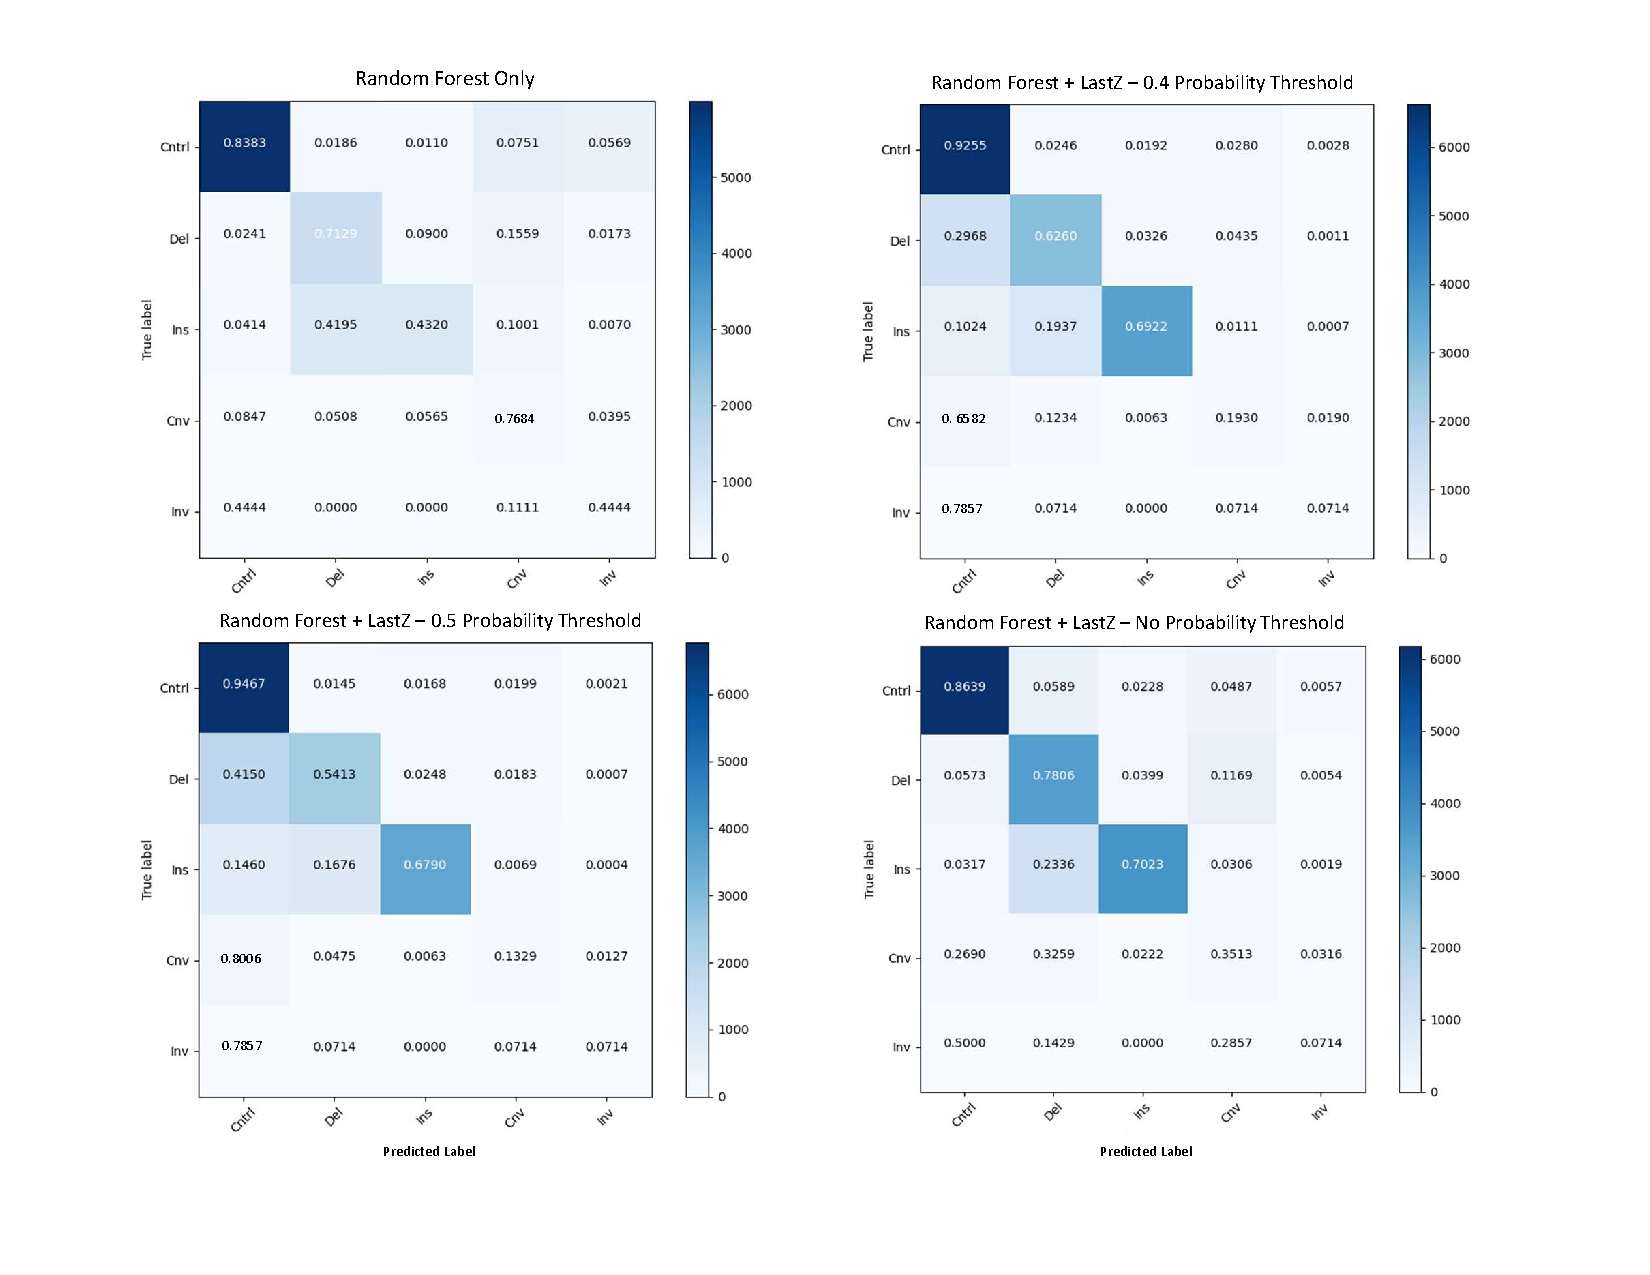
\includegraphics[width=1.2\textwidth]{figures/ch3/thresholding.pdf}}
    \caption[Random Forest caller accuracy with and without prior candidate regions.]{Random Forest caller accuracy with and without prior candidate regions. Labels are controls, deletion, insertions, copy number variants, and inversions, respectively. Values are reported as proportion of true labels (along the y-axis) that are included in a given intersection. Color indicates number of samples in a given intersection scaled to the largest number of samples in a class.}
    \label{fig:caller_comparison}
\end{figure}

\subsection{SV detection remains a challenging task with object detection frameworks}

We attempted to use an object detection framework (YOLOv5) on an alternative feature vector representation of SVs and their breakpoints. Breakpoint identification is attractive as opposed to whole-SV detection due to its lower computational cost both in terms of creating a feature vector (less genomic information needs to be loaded into memory at any given point), but also during training/testing of a model. An additional benefit of breakpoint identification is complex SV structures, where a single breakpoint is involved with multiple SV events (a duplication followed by an inversion, for example). Though the whole-SV detection approach allows for an overall easier workflow as no breakpoint matching needs to be done, it is extremely resource intensive, often impossible to fit an entire SV in an "image" with our proposed feature vector \ref{fig:example_pileup}. We found no significant ability to detect either breakpoints or SVs using this approach, leading us to the conclusion that alternative approaches to either feature engineering, choice of model, or both are necessary to accomplish this task. 

\section{Discussion}

We attempted to classify and discover structural variants using random forests and state of the art object detection models with a set of long-read and short-read matched sequencing assemblies of \textit{Drosophila melanogaster}. We find that our feature engineering and random forest approach is highly accurate as a filtering mechanism for genotyping candidate SVs, however detection from no prior knowledge or candidates remains a challenging task in the field. We propose that with further work into more computationally efficient feature engineering and alternative approaches to object detection our work could be useful in the context of population-scale short-read structural variant calling, allowing for the use of SVs in population genetics analyses where it was previously infeasible. 